\documentclass{beamer}
%
% Choose how your presentation looks.
%
% For more themes, color themes and font themes, see:
% http://deic.uab.es/~iblanes/beamer_gallery/index_by_theme.html
%
\mode<presentation>
{
  \usetheme{default}      % or try Darmstadt, Madrid, Warsaw, ...
  \usecolortheme{default} % or try albatross, beaver, crane, ...
  \usefonttheme{default}  % or try serif, structurebold, ...
  \setbeamertemplate{navigation symbols}{}
  \setbeamertemplate{caption}[numbered]
}

\usepackage[english]{babel}
\usepackage[utf8]{inputenc}
\usepackage[T1]{fontenc}

\newcommand{\emphbf}[1]{\textbf{\emph{#1}}}

\title[Graphics Pipeline]{The Real-Time Graphics Pipeline}
\author{Benjamin Brown}
%\institute{Where You're From}
\date{Monday, 26th September 2022}

\begin{document}

\begin{frame}
  \titlepage
\end{frame}

% Uncomment these lines for an automatically generated outline.
%\begin{frame}{Outline}
%  \tableofcontents
%\end{frame}

\begin{frame}{The Key Idea}

Basic task in computer graphics is \emphbf{render} 3-dimensional objects:

\begin{itemize}
  \item given a scene composed of geometric objects in 3d space;
  \item produce a 2d image showing the objects from a specific viewpoint.
\end{itemize}

\vskip 1cm

Two methods of rendering:

\begin{itemize}
	\item \emphbf{object-order rendering}: for each \textcolor{blue}{object}, which \textcolor{red}{pixels} are influenced by it?
		\begin{itemize}
			\item Example: rasterisation.
		\end{itemize}
	\item \emphbf{image-order rendering}: for each \textcolor{red}{pixel}, which \textcolor{blue}{object} is influenced by it?
		\begin{itemize}
			\item Example: ray-tracing.
		\end{itemize}
\end{itemize}

\end{frame}

\begin{frame}{Real-Time Rendering}

	\emphbf{Real-time rendering} refers to the process of rendering a scene in less than 1/30\textsuperscript{th} of a second (i.e., refresh rate $>$ 30 Hz).

	\begin{itemize}
		\item Real-time rendering refers to rendering that is fast enough to allow for the user's \emphbf{real-time interaction}.
		\item As little as 15 ms of temporal delay can slow and interfere with the interactivity.
	\end{itemize}

	\vskip 1cm

	So speed is essential for interactivity:

	\begin{itemize}
		\item For a 1080p image at 90 Hz, an image-order rendering iteration would need to be performed 186,624,000 times per second.
		\item Object-order rendering is (usually) faster in this case.
	\end{itemize}

\end{frame}

\begin{frame}{The Graphics Pipeline}

	The main function of the \emphbf{graphics pipeline} is:

	\begin{itemize}
		\item Given a virtual camera, 3d objects, light sources, etc., render a 2d image;
		\item Object locations and shapes determined by their geometry, environment,  camera placement, etc.;
		\item Object appearance affected by material, light sources, shading, etc.
	\end{itemize}

	\vskip 1cm

	Some key ideas regarding the pipeline are:

	\begin{itemize}
		\item Consists of several states, with each making up part of a larger task;
		\item The states execute in parallel, with each stage dependent on the result from the previous.
	\end{itemize}

\end{frame}

\begin{frame}{Stages of the Graphics Pipeline}

	Roughly, the main stages of the pipeline are:

	\begin{enumerate}
		\item \emphbf{application};
		\item \emphbf{geometry processing};
		\item \emphbf{rasterisation};
		\item \emphbf{pixel processing}.
	\end{enumerate}

	\vskip 1cm

	\begin{figure}[t]
		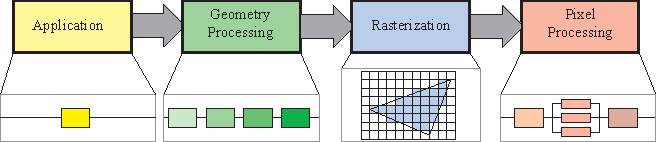
\includegraphics[width=8cm]{main-pipeline}
		\centering
	\end{figure}

\end{frame}

\begin{frame}{The Application Stage}

	Involves tasks typically implemented by the software running on general-purpose CPUs:

	\begin{itemize}
		\item collision detection;
		\item animation;
		\item physics simulation, etc...
	\end{itemize}

	\vskip 1cm

	More specifically, the application stage:

	\begin{itemize}
		\item Reads \emphbf{primitive} data and assembles it into primitives for later states.
		\begin{itemize}
			\item Vertex data (position, normal vectors, colour, etc.),
		\end{itemize}
		\item Initialises GPU allocated memory buffers.
		\begin{itemize}
			\item Vertex and index buffers.
		\end{itemize}
	\end{itemize}

\end{frame}

\begin{frame}{The Geometry Processing Stage}

	Responsible for the per-triangle and per-vertex operations:

	\begin{itemize}
		\item Vertex processing (transforming and shading);
		\item Projecting;
		\item Clipping;
		\item Screen mapping.
	\end{itemize}

	\vskip 1cm

	\begin{figure}[t]
		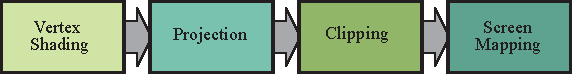
\includegraphics[width=8cm]{geometry-pipeline}
		\centering
	\end{figure}

\end{frame}

\begin{frame}{The Geometry Processing Stage}

	\emphbf{Vertex shading} deals with:

	\begin{itemize}
		\item Determining the effect of a light on a material (\emphbf{shading});
		\item Projecting from \emphbf{world space} onto \emphbf{view space};
		\item \emphbf{Clipping} away the view space primitives which do not lie within the view volume;
		\item Mapping the vertices onto \emphbf{screen space};
	\end{itemize}

	\vskip 1cm

	\begin{itemize}
		\item
	\end{itemize}

\end{frame}

\begin{frame}{Rasteristaion}

	The \emphbf{rasterisation} stage converts vector information (composed of primitives) into a raster image (composed of pixels). It includes:

	\begin{itemize}
		\item Dividing by $z$ for perspective;
		\item Mapping primitives to a 2D viewport;
		\item Determining how to invoke the pixel.
	\end{itemize}

	\vskip 1cm

	\begin{itemize}
		\item
	\end{itemize}

\end{frame}


\begin{frame}{Tables and Figures}

\begin{itemize}
\item Use \texttt{tabular} for basic tables --- see Table~\ref{tab:widgets}, for example.
\item You can upload a figure (JPEG, PNG or PDF) using the files menu.
\item To include it in your document, use the \texttt{includegraphics} command (see the comment below in the source code).
\end{itemize}

\begin{block}{Examples}
	Some examples of commonly used commands and features are included, to help you get started.
\end{block}

% Commands to include a figure:
%\begin{figure}
%\includegraphics[width=\textwidth]{your-figure's-file-name}
%\caption{\label{fig:your-figure}Caption goes here.}
%\end{figure}

\begin{table}
\centering
\begin{tabular}{l|r}
Item & Quantity \\\hline
Widgets & 42 \\
Gadgets & 13
\end{tabular}
\caption{\label{tab:widgets}An example table.}
\end{table}

\end{frame}

\begin{frame}{Readable Mathematics}

Let $X_1, X_2, \ldots, X_n$ be a sequence of independent and identically distributed random variables with $\text{E}[X_i] = \mu$ and $\text{Var}[X_i] = \sigma^2 < \infty$, and let
\[ S_n = \frac{X_1 + X_2 + \cdots + X_n}{n}
      = \frac{1}{n}\sum_{i}^{n} X_i \]
denote their mean. Then as $n$ approaches infinity, the random variables $\sqrt{n}(S_n - \mu)$ converge in distribution to a normal $\mathcal{N}(0, \sigma^2)$.

\end{frame}

\end{document}
